%
% gauss.tex -- Gauss
%
% (c) 2021 Prof Dr Andreas Müller, OST Ostschweizer Fachhochschule
%
\bgroup
\begin{frame}[t]
\setlength{\abovedisplayskip}{5pt}
\setlength{\belowdisplayskip}{5pt}
\frametitle{Satz von Gauss}
\begin{center}
\begin{tikzpicture}[>=latex]
\uncover<2>{
	\node at (0,0) {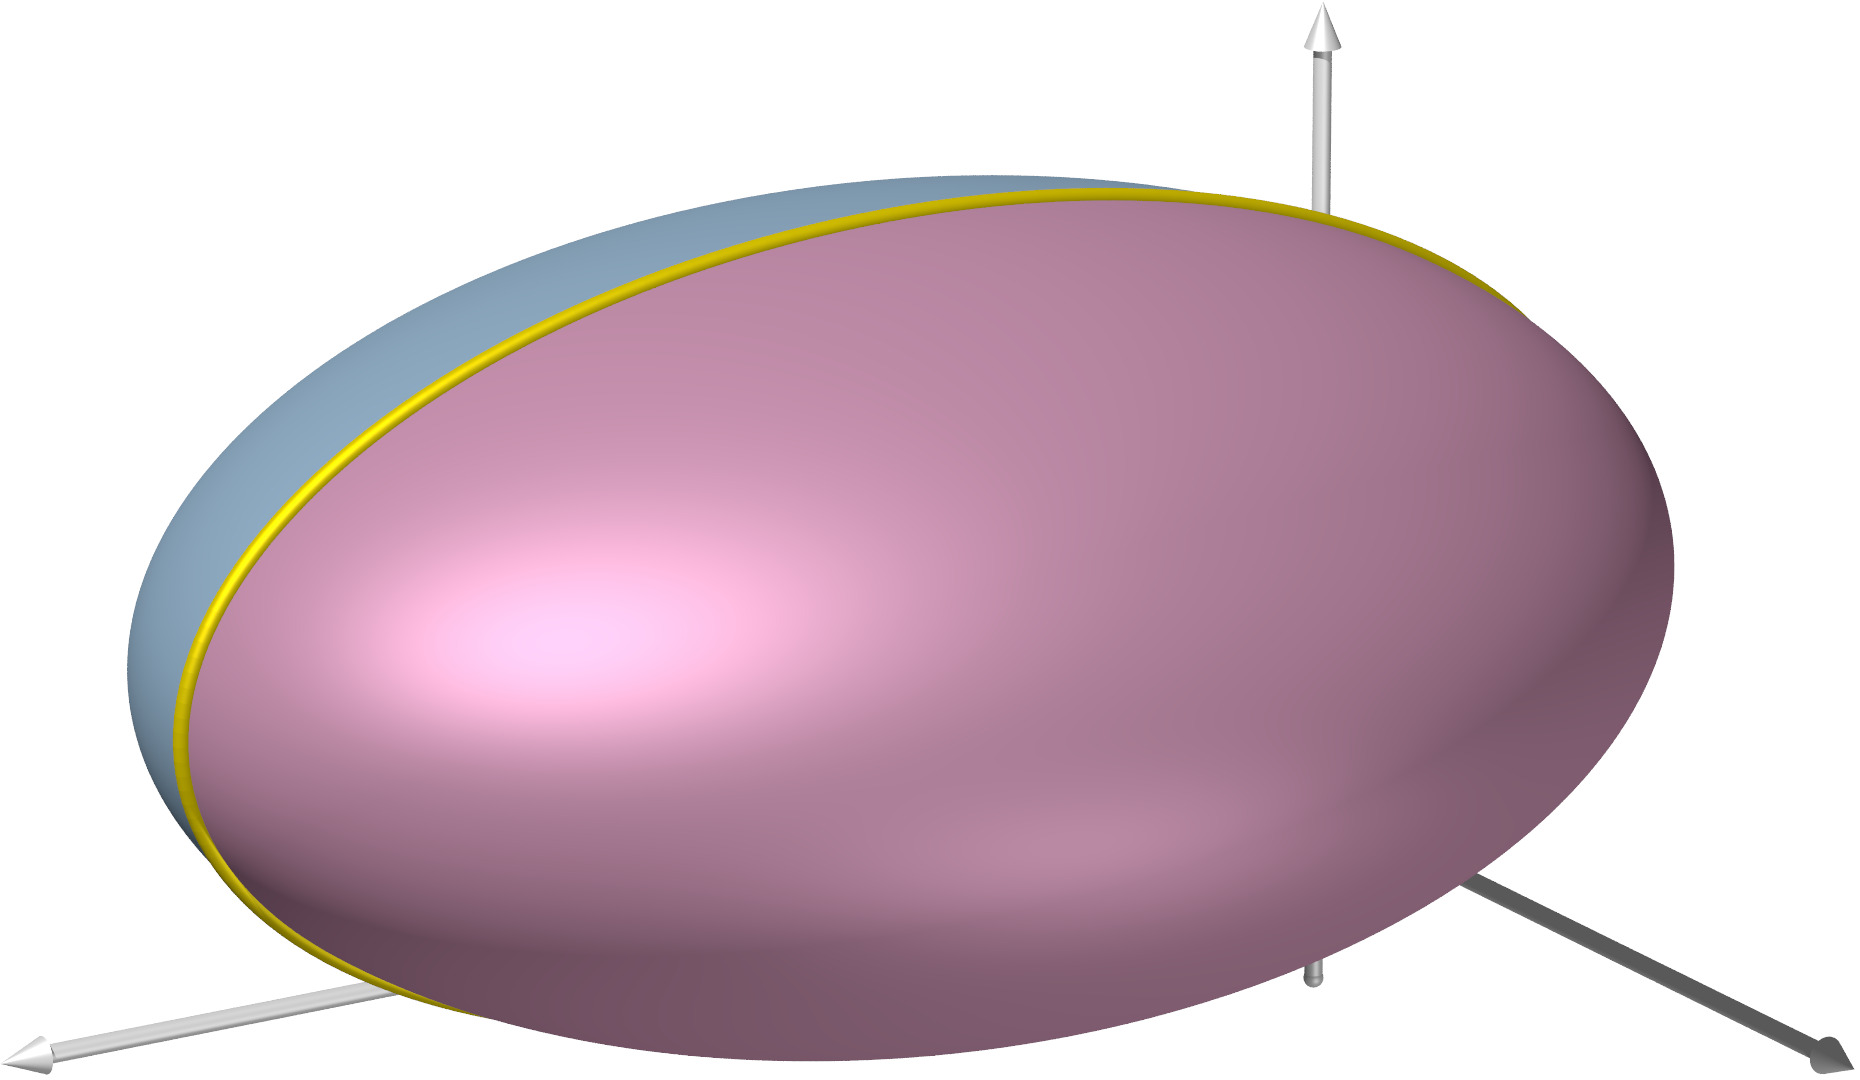
\includegraphics[width=12cm]{../slides/5/gaussy.jpg}};
	\node at (0,-1) {$y_+(x,z)$};
	\node at (-3.6,1.4) {$y_-(x,z)$};
}
\uncover<3>{
	\node at (0,0) {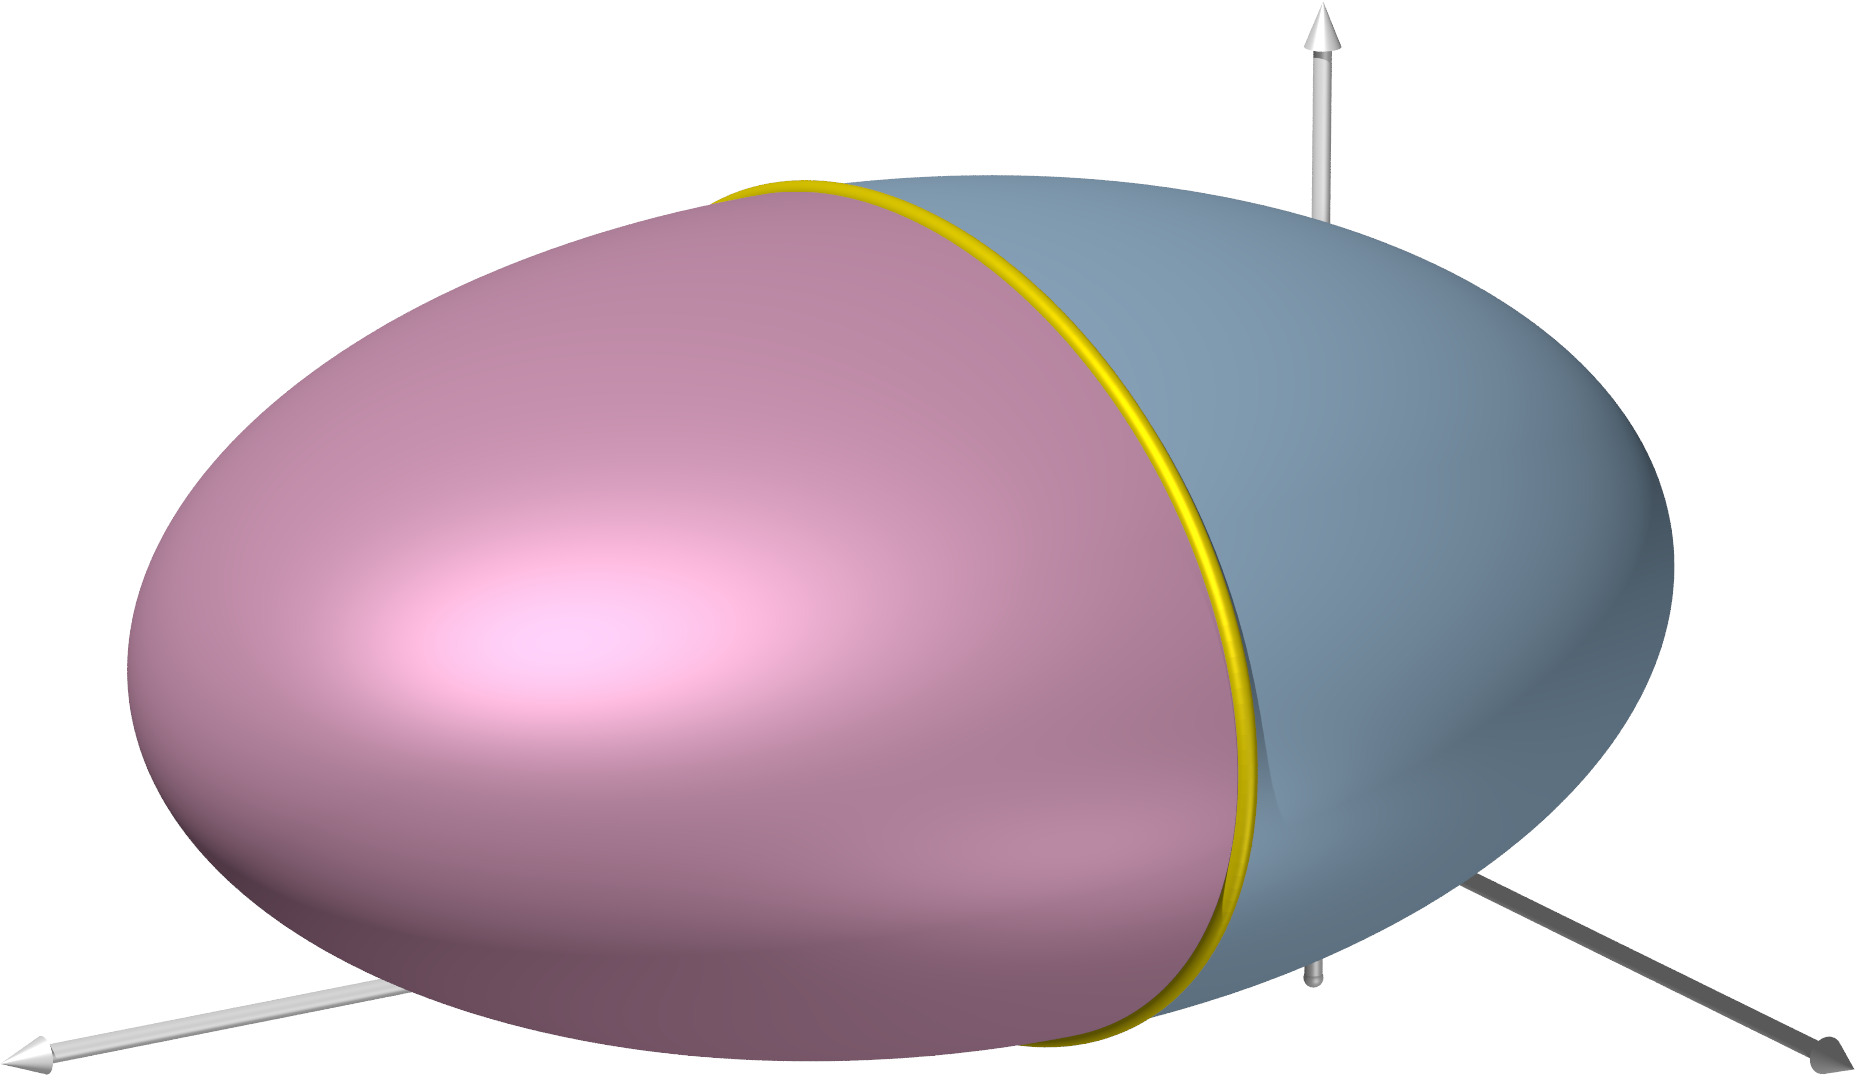
\includegraphics[width=12cm]{../slides/5/gaussx.jpg}};
	\node at (-2,-1) {$x_+(y,z)$};
	\node at (3,0) {$x_-(y,z)$};
}
\uncover<1>{
	\node at (0,0) {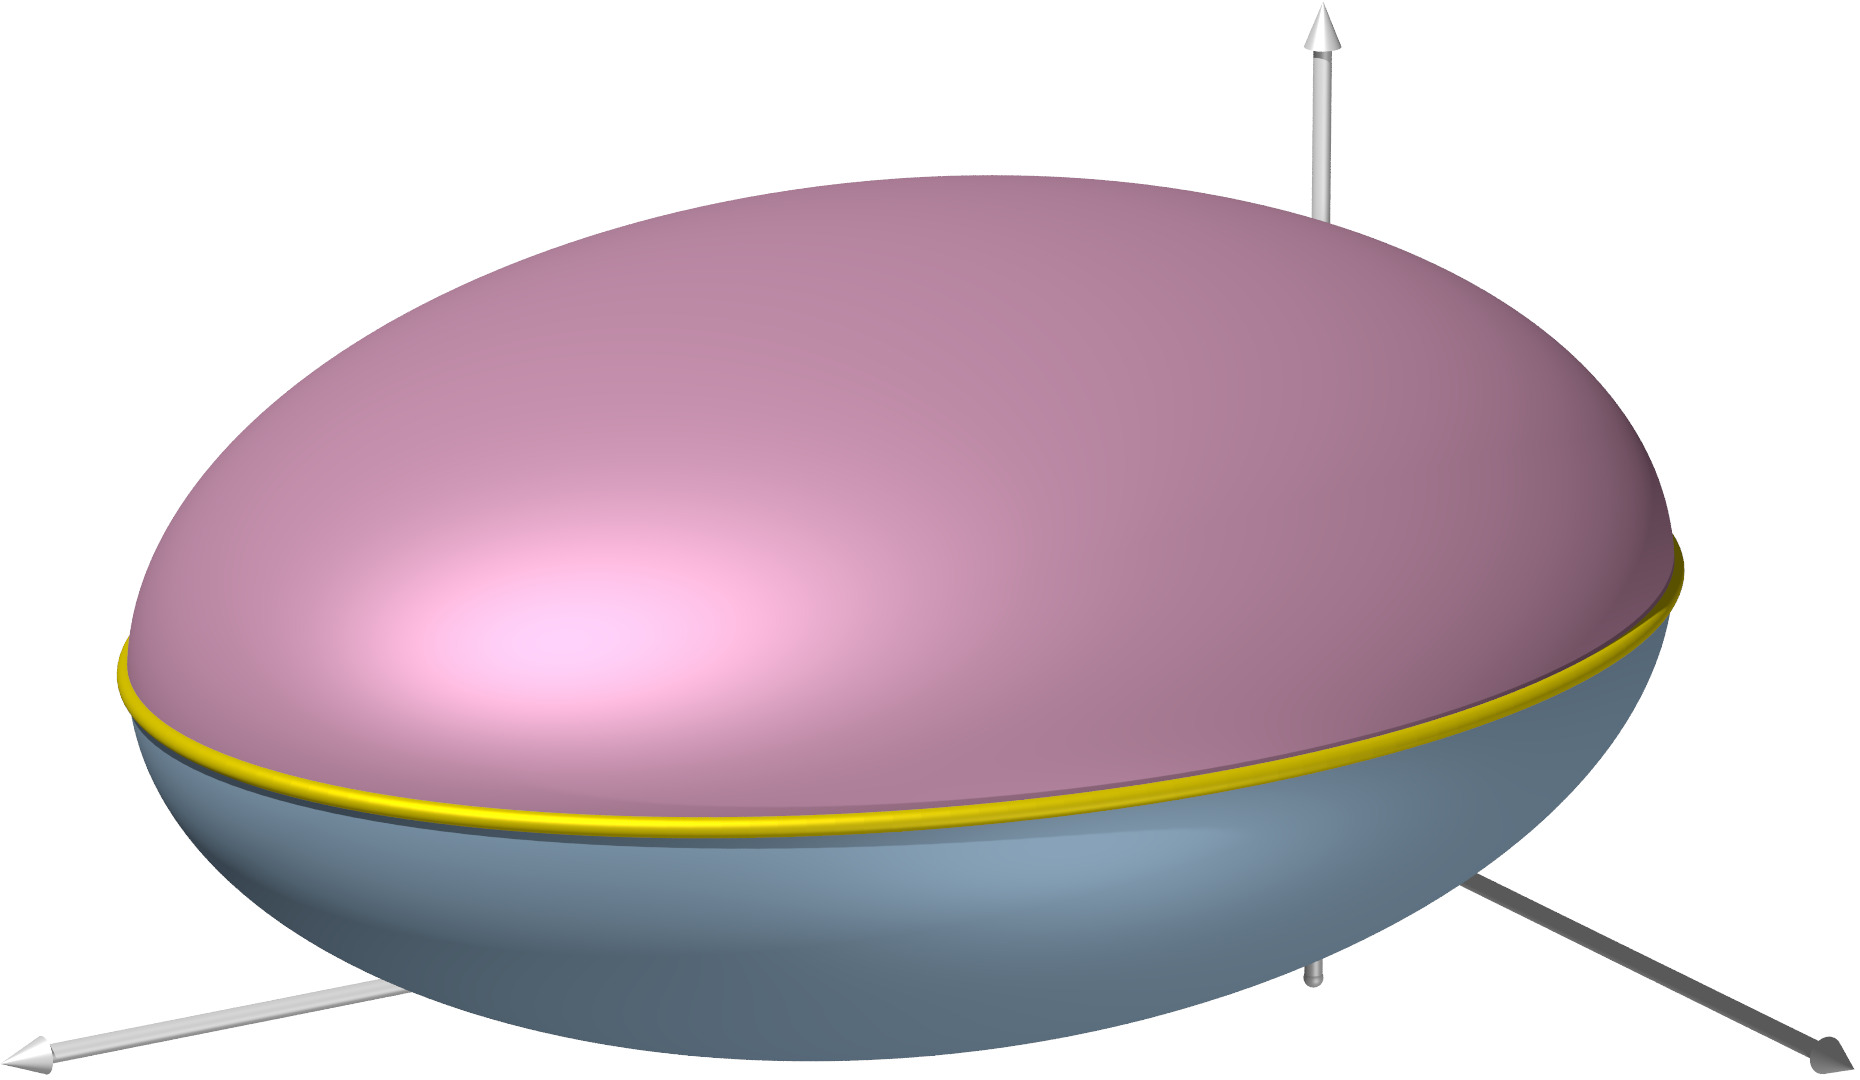
\includegraphics[width=12cm]{../slides/5/gaussz.jpg}};
	\node at (0,0) {$z_+(x,y)$};
	\node at (0,-2.5) {$z_-(x,y)$};
}
\node at (-5.8,-3) {$x$};
\node at (5.8,-3) {$y$};
\node at (2.9,3.3) {$z$};
\end{tikzpicture}
\end{center}
\end{frame}
\egroup
